\section{Convergence graph}

We first take a look at the converging predicted energy for the Pairing model with $P = 12$ energy levels included, $n = 6$ particle pairs, $\varepsilon = -0.3$ and $g = -1$.

\begin{figure}[H]
  \begin{center}
    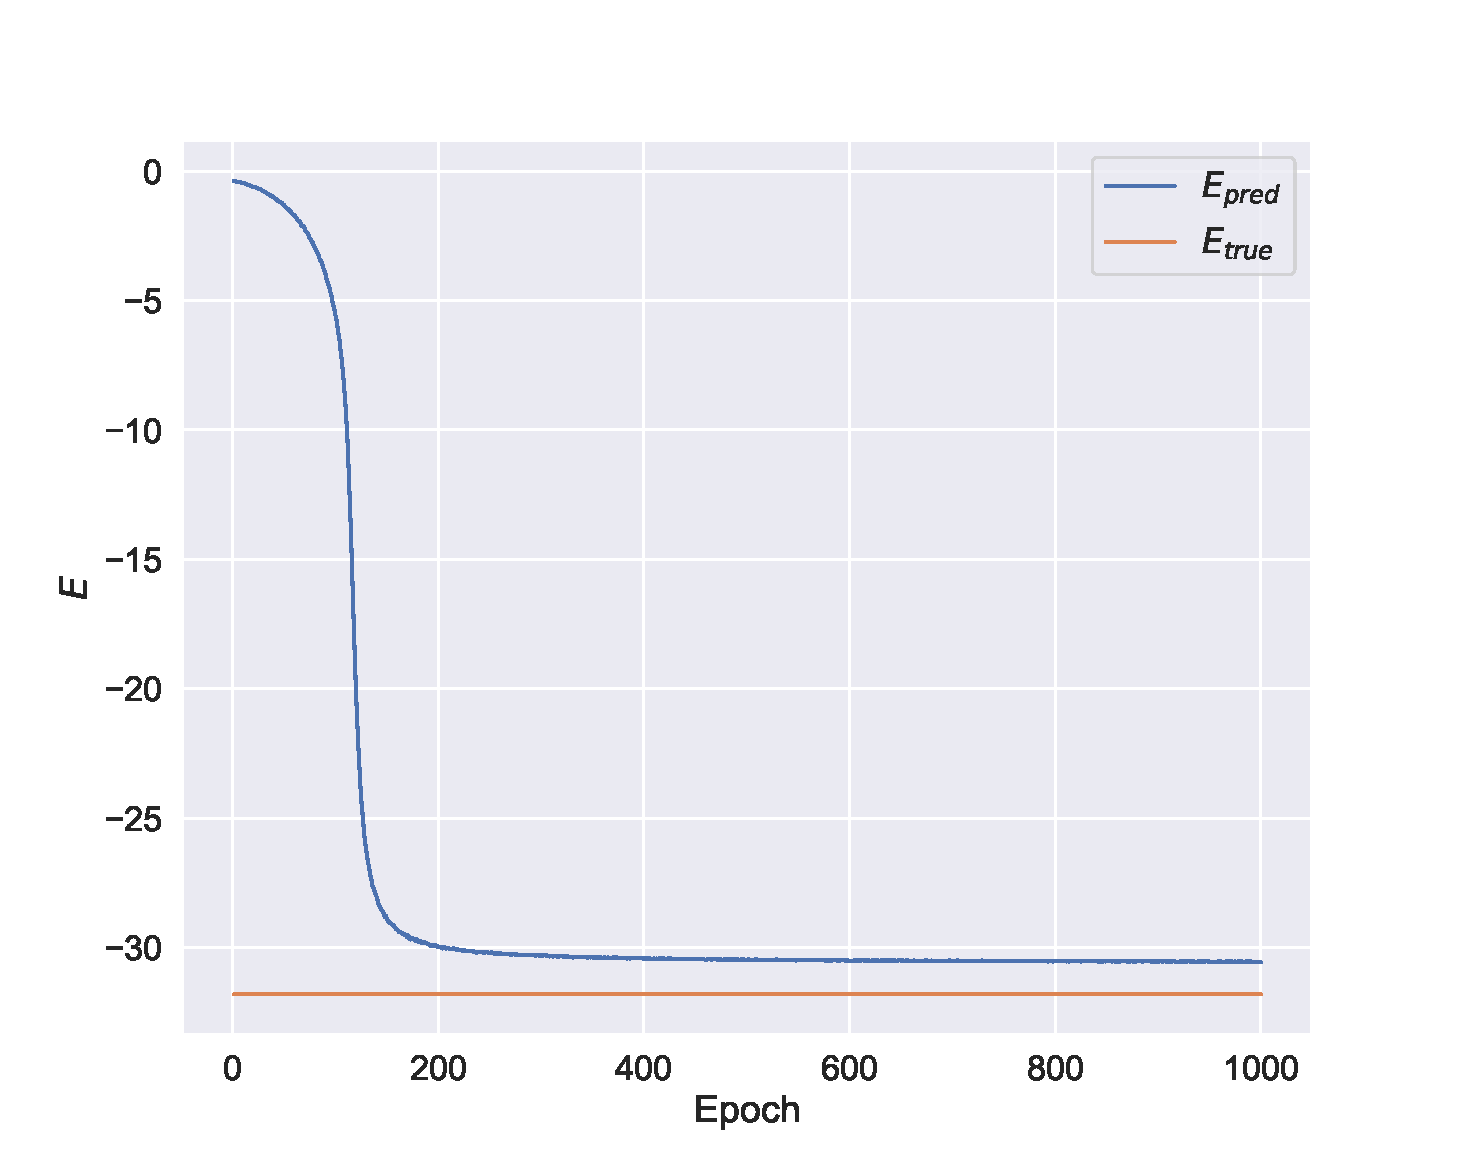
\includegraphics[width=0.95\textwidth]{Figures/Plots/Pairing/pairing_conv12}
  \end{center}
  \caption{The convergence graph of the RBM mean energy output for the Pairing model with particle pairs $n = 6$, levels $P=12$, and $\varepsilon=-0.3$ and $g=-1$.}
\end{figure}

Here we too have a small gap between the true ground state energy and the energy the RBM converge towards. This does as said earlier suggest that the RBM doesn't find the true wavefunction. 

\subsection{The effect of \texorpdfstring{$\varepsilon$}{epsilon} on RBM prediction accuracy}

Taking a look at the single particle energy variable $\varepsilon$ with a system of included energy levels $P = 10$, particles $n = 5$ and $g = 0$, we get:

\begin{figure}[H]
  \begin{center}
    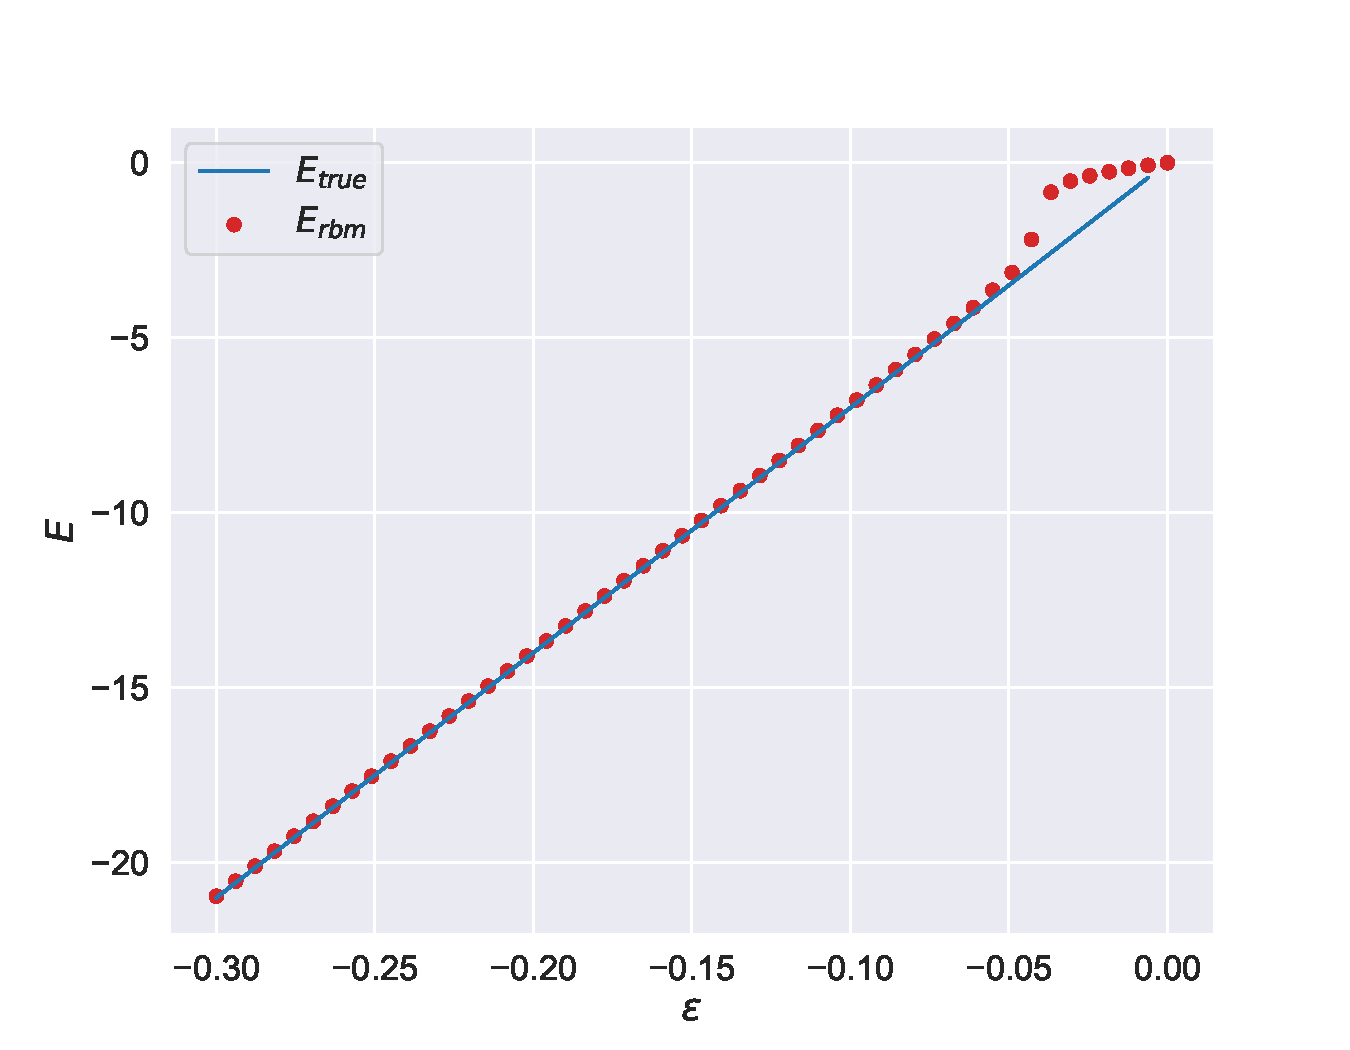
\includegraphics[width=0.95\textwidth]{Figures/Plots/Pairing/val-true[eps][-0.3-0.0][e=1000][n=10][n=5][g=0]}
  \end{center}
  \caption{The accuracy of the RBM for different values of $\varepsilon$ with number of particles as $n = 5$, levels $P=10$, and $g=0$.}
\end{figure}

The RBM seem to match the true ground state well for values up to $\varepsilon = -0.05$. At this point the RBM's predicted energy jumps closer to zero. For the Pairing model the Hamiltonian matrix does have large parts zeroed out, as many of the basis state are not accessible, and the RBM has to manage to find the accessible states by the lower local energy. Past a threshold a too small $\varepsilon$ may make these too difficult to distinguish.

\subsection{The effect of particle pairs on RBM accuracy}

We can then change the number of particle pairs instead, fixing $\varepsilon = -0.3$.

\begin{figure}[H]
  \begin{center}
    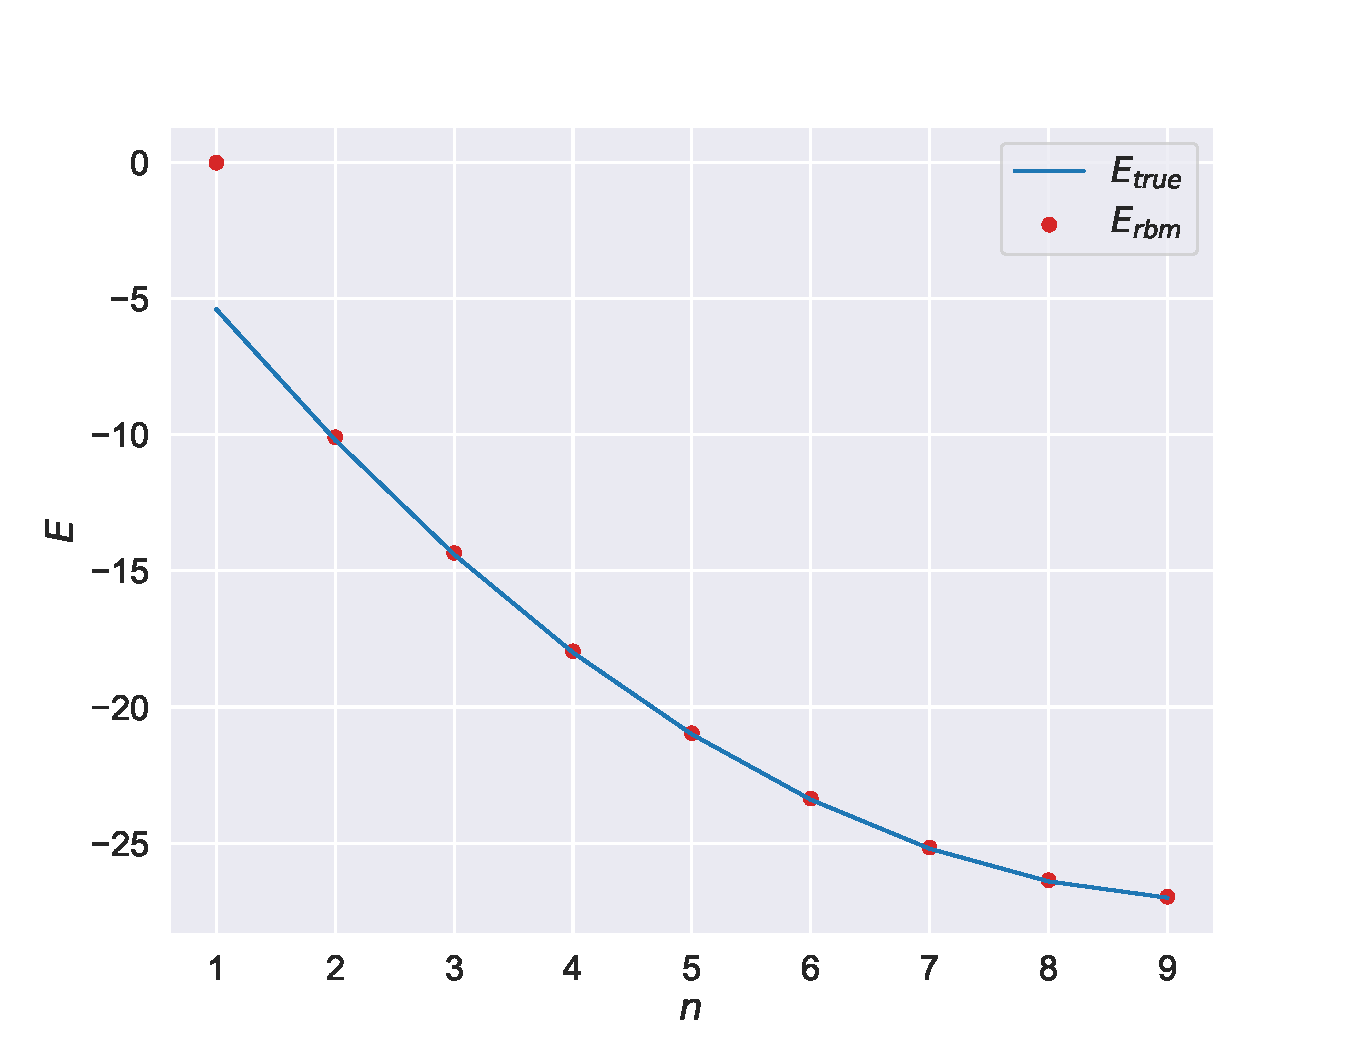
\includegraphics[width=0.95\textwidth]{Figures/Plots/Pairing/val-true[particles][1-9][e=1000][n=9][eps=-0.3][g=0]}
  \end{center}
  \caption{The accuracy of the RBM for different values of $\varepsilon$ with number of particles as $\eps = -0.3$, levels $P=10$, and $g = 0$.}
\end{figure}

The RBM predictors the ground state accurately for the different numbers of particle pairs except for $n=1$ where it defaults back to $E_{rbm} = 0$. A cause may be that for the case of only one particle pair the Hamiltonian matrix contains almost only zeros, so the RBM struggles to find the accessible states. This begs the question why the RBM manages to predict the ground state energy accurately for the $n=9$ case, where the number of non-accessible basis states are the same as for $n=1$. As suggested previously this may come from that the energy for $n=9$ case is of higher absolute value, such that additions of the accessible basis states in the machine state has a larger effect on the machine state energy during the learning process.

\subsection{The effect of \texorpdfstring{$g$}{g} on RBM prediction accuracy}

\begin{figure}[H]
  \begin{center}
    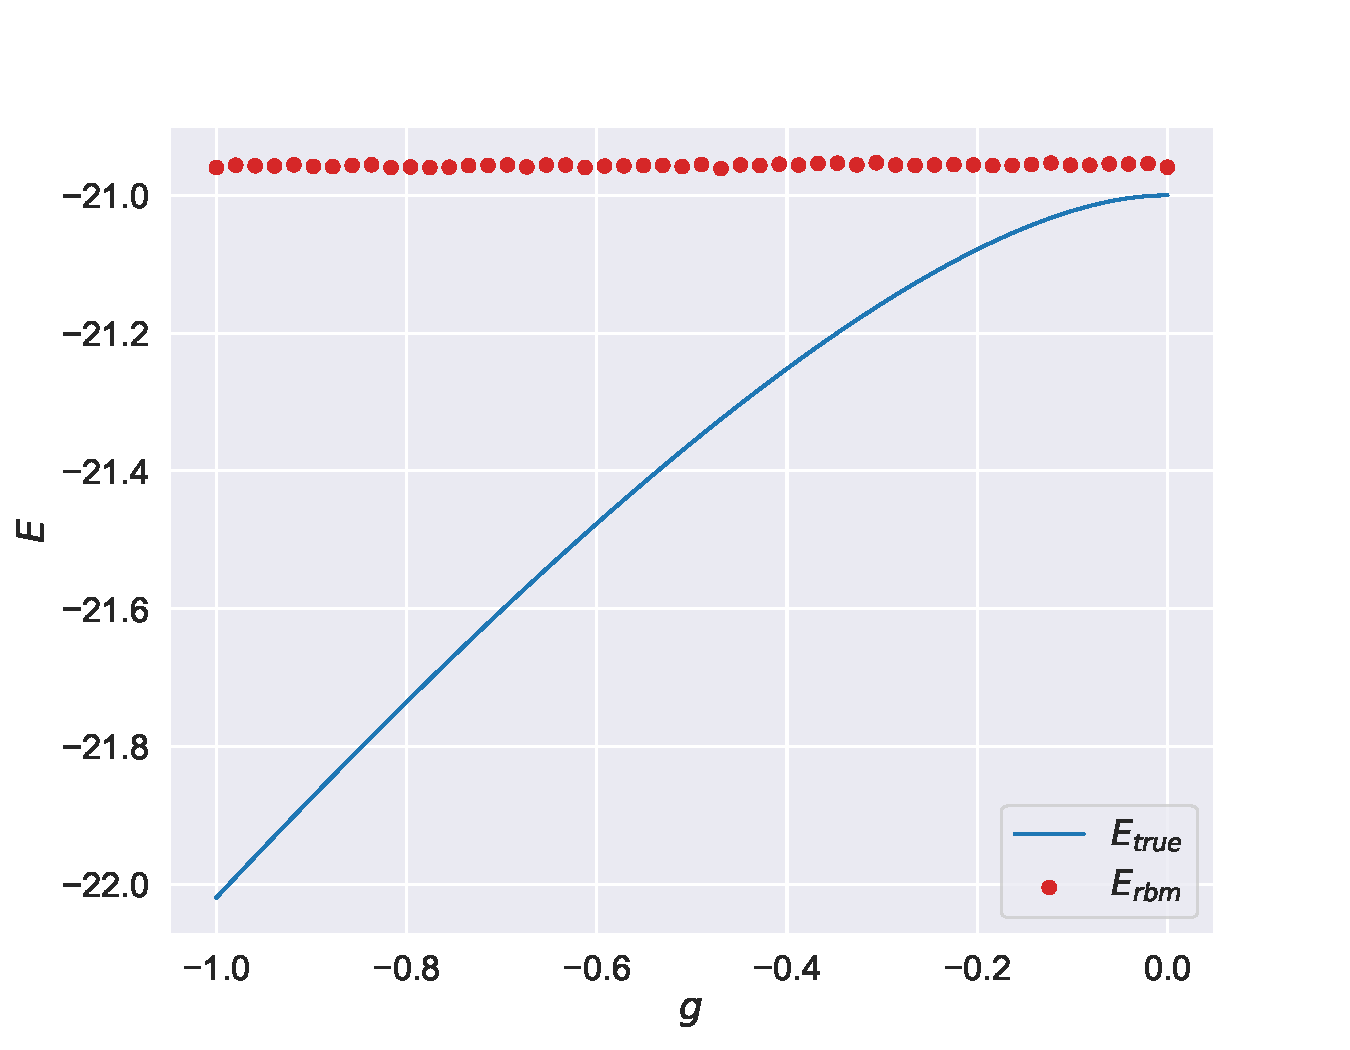
\includegraphics[width=0.95\textwidth]{Figures/Plots/Pairing/val-true[g][-1.0-0.0][e=1000][n=10][n=5][eps=-0.3]}
  \end{center}
  \caption{The accuracy of the RBM for different values of $\varepsilon$ with number of particles as $\eps = -0.3$, $n=5$ and levels $P=10$.}
\end{figure}

It is clear that the restricted Boltzmann machine completely ignores the $g$ interaction strength of the Pairing model. A reason for this may be that it finds the non-interactive ground state energy, but then struggles to escape the local minima or that the local energy average becomes too sensitive to small changes to the machine state.

